\chapter{Slice Testing}

The long-term goal of this work is to create an integrated biosensor for use with living cells. Thus, proof-of-concept tests were performed. These were done by preparing a chip with the PDMS well, doing a basic test to determine if the chip was working (although not how well it worked), and attaching a living slice of a mouse ovary to the surface of the chip, over the sensor sites. Care was taken to ensure the slice would stay living up to and during the tests by keeping it at a temperature of $37\,^{\circ}\mathrm{C}$, and submerged in neurobasal. After the ovary slice was attached the chip was moved into a different lab. The temperature was measured by lowering the end of a thermometer below the surface of the neurobasal, and heated with a lamp to the appropriate temperature (Figure \ref{slice-top}). The entire testing device was enclosed in a Faraday cage. Previously, a chip had been prepared in the same fashion, but with no ovary, and tested with the lamp on. This test showed that the lamp did not contribute noise to the results.

After these preparations, the chip was connected to the 660B potentiostat at sensor 17, working electrode 41. Amperometry was performed at 0.85V for 30 minutes. Compared to \cite{mosharok2005aee} (Figure \ref{amperometric-pulses}), we see that our results are consistent with the release profile. Both exhibit a sharp change, followed by an exponential decrease back to the baseline.

\begin{figure}
	\centering
	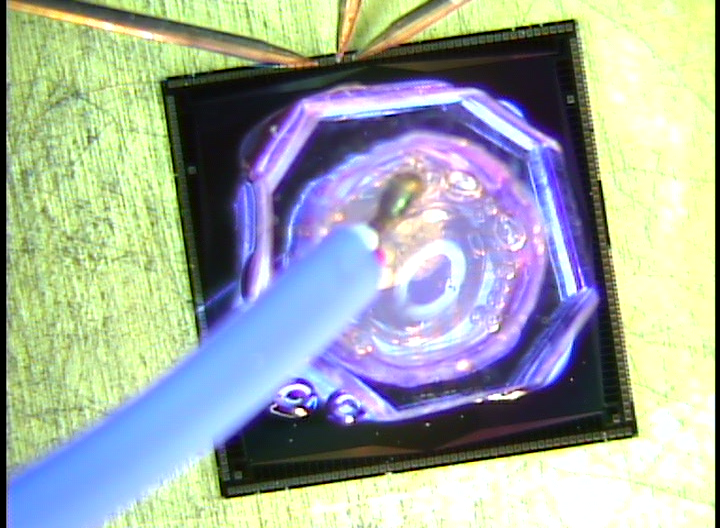
\includegraphics[width=\linewidth]{figures/slice-top.png}
	\caption[Top view of chip under testing with an ovary slice attached.]{Top view of chip under testing with an ovary slice attached. The blue wire is a temperature sensor.}
	\label{slice-top}
\end{figure}

\begin{figure}
	\centering
	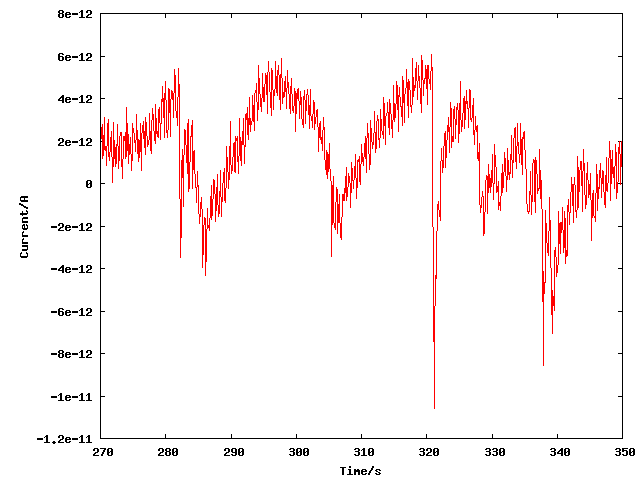
\includegraphics[width=0.7\linewidth]{figures/216.png}
	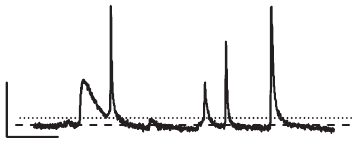
\includegraphics[width=0.7\linewidth]{figures/mosharok-pulse.png}
	\caption[Amperometric pulses.]{Amperometric pulses from two separate tests. Top: from ovary-slice test. Bottom: figure 2 (a) of \cite{mosharok2005aee}. Scale bars, 50 pA and 100 ms for the timescale.}
	\label{amperometric-pulses}
\end{figure}
